\documentclass{ximera}

\input{../../../preamble.tex}


\definecolor{fvdnavy}{HTML}{071D43}
\definecolor{fvdcyan}{HTML}{20BFC6}
\definecolor{fvdcyanlight}{HTML}{EFFCFB}
\definecolor{fvdmagenta}{HTML}{F10D69}
\definecolor{fvdmagentalight}{HTML}{FFF1F7}
\definecolor{fvdtext}{HTML}{163044}





%=================================================
% Pedagogische omgevingen
% PDF: tcolorbox
% HTML: learning-box
%=================================================

\newenvironment{voorkennis}
{%
    \ifdefined\HCode
        \HCode{%
<section class="learning-box learning-box--prior">
<div class="learning-box__header">
<span class="learning-box__icon" aria-hidden="true"></span>
<span class="learning-box__title">Voorkennis</span>
</div>
<div class="learning-box__content">
        }%
        \begin{itemize}
    \else
       \begin{tcolorbox}[
    enhanced,
    breakable,
    colback=fvdcyanlight,
    colframe=fvdcyan,
    coltext=fvdtext,
    boxrule=0.5pt,
    leftrule=4pt,
    arc=4mm,
    outer arc=4mm,
    left=7mm,
    right=6mm,
    top=5mm,
    bottom=5mm,
    before skip=6mm,
    after skip=6mm,
    title=Voorkennis,
    coltitle=fvdcyan,
    fonttitle=\bfseries\Large,
    attach title to upper={\par\smallskip},
    boxed title style={
        empty,
        left=0mm,
        right=0mm,
        top=0mm,
        bottom=0mm
    },
    overlay={
        \draw[
            fvdcyan,
            line width=0.5pt
        ]
        ([xshift=42mm,yshift=-13mm]frame.north west)
        --
        ([xshift=-7mm,yshift=-13mm]frame.north east);
    }
]
        \begin{itemize}
    \fi
}
{%
    \end{itemize}
    \ifdefined\HCode
        \HCode{%
</div>
</section>
        }%
    \else
        \end{tcolorbox}
    \fi
}


\newenvironment{leerdoelen}
{%
    \ifdefined\HCode
        \HCode{%
<section class="learning-box learning-box--goals">
<div class="learning-box__header">
<span class="learning-box__icon" aria-hidden="true"></span>
<span class="learning-box__title">Leerdoelen</span>
</div>
<div class="learning-box__content">
        }%
        \begin{itemize}
    \else
\begin{tcolorbox}[
    enhanced,
    breakable,
    colback=fvdmagentalight,
    colframe=fvdmagenta,
    coltext=fvdtext,
    boxrule=0.5pt,
    leftrule=4pt,
    arc=4mm,
    outer arc=4mm,
    left=7mm,
    right=6mm,
    top=5mm,
    bottom=5mm,
    before skip=6mm,
    after skip=6mm,
    title=Leerdoelen,
    coltitle=fvdmagenta,
    fonttitle=\bfseries\Large,
    attach title to upper={\par\smallskip},
    boxed title style={
        empty,
        left=0mm,
        right=0mm,
        top=0mm,
        bottom=0mm
    },
    overlay={
        \draw[
            fvdmagenta,
            line width=0.5pt
        ]
        ([xshift=42mm,yshift=-13mm]frame.north west)
        --
        ([xshift=-7mm,yshift=-13mm]frame.north east);
    }
]
        \begin{itemize}
    \fi
}
{%
    \end{itemize}
    \ifdefined\HCode
        \HCode{%
</div>
</section>
        }%
    \else
        \end{tcolorbox}
    \fi
}



\title{Domein, bereik, beelden en originelen}
\author{Ingmar Herreman}

\begin{document}

% FVD_CHAPTER_DATA_START
% Automatisch gegenereerd uit index.tex.
% Niet handmatig aanpassen.
\fvdchapterdata{4}{Van relatie naar functie}{2}
% FVD_CHAPTER_DATA_END









\begin{abstract}
Een functie koppelt invoerwaarden aan uitvoerwaarden. Maar welke invoerwaarden
zijn toegelaten? Welke uitvoerwaarden worden werkelijk bereikt? En hoe lezen we
dit af uit een voorschrift, een grafiek of een concrete situatie?

In dit hoofdstuk bouwen we de taal op die we later voortdurend nodig hebben:
\textbf{domein}, \textbf{bereik}, \textbf{beeld} en \textbf{origineel}.
We leren deze begrippen grafisch, algebraïsch en in context gebruiken.
Grafieken en GeoGebra zijn daarbij onderzoeksgereedschap, niet alleen illustratie.
\end{abstract}

\maketitle

\begin{voorkennis}
    \item Je begrijpt wanneer een relatie een functie is.
    \item Je kan werken met functienotatie \(f(x)\).
    \item Je kan functiewaarden berekenen.
    \item Je kan eenvoudige grafieken en intervallen lezen.
\end{voorkennis}

\begin{leerdoelen}
    \item Je kan het domein en bereik van een functie uitleggen en noteren.
    \item Je kan domein en bereik uit een grafiek aflezen.
    \item Je kan bij eenvoudige voorschriften het domein bepalen vanuit de algebraïsche voorwaarden.
    \item Je kan onderscheid maken tussen een wiskundig domein en een domein dat door een context wordt beperkt.
    \item Je kan beelden berekenen en grafisch bepalen.
    \item Je kan originelen grafisch en algebraïsch bepalen.
    \item Je begrijpt dat één beeld meerdere originelen kan hebben.
    \item Je kan domein, bereik, beelden en originelen interpreteren in een betekenisvolle situatie.
    \item Je kan GeoGebra gebruiken om deze kenmerken van een functie te onderzoeken.
\end{leerdoelen}



% ============================================================
% 1. DOMEIN
% ============================================================

\FVDsection{Het domein}
\FVDsubsection{Welke invoerwaarden zijn mogelijk?}

In het vorige hoofdstuk beschreven we een functie als een relatie waarbij iedere
\emph{toegelaten} invoerwaarde precies één uitvoerwaarde krijgt. Het woord
``toegelaten'' verdient nu onze aandacht.

\begin{definitie}
Het \textbf{domein} van een functie \(f\) is de verzameling van alle
invoerwaarden waarvoor de functie gedefinieerd is.

We noteren bijvoorbeeld
\[
\operatorname{dom}f.
\]
\end{definitie}

\begin{center}
    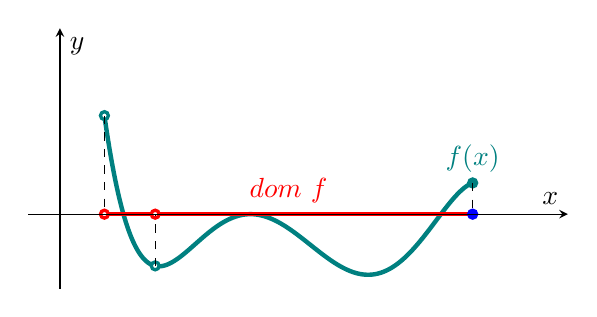
\begin{tikzpicture}

        \begin{axis}[
                    xlabel={$x$},
                    ylabel={$y$},
                    axis equal image=true,
                    grid,
                    grid style={gray!50},
                    grid=both,
                axis y line=center,
                axis x line=middle, 
                axis on top=true,
                xmin=-0.5,
                xmax=8,
                ymin=-2,
                ymax=5,
                xtick={\empty},
                ytick={\empty},
                x=6 cm,
                    ]
            \addplot [domain=0.7:6.5, samples=500, mark=none, ultra thick, teal] {-0.05*(x-1)*(x-3)*(x-3)*(x-6)*(x-7)};
            \draw[red,ultra thick] (axis cs: 0.7,0) -- (axis cs: 6.5,0) node[midway,above] {$dom \ f$};
            \draw[teal, very thick,fill=white]  (axis cs: 0.7,2.65) circle (0.5 mm);
            \draw[red, very thick,fill=white]  (axis cs: 0.7,0) circle (0.5 mm);
            \draw[teal, very thick,fill=white]  (axis cs: 1.5,-1.39) circle (0.5 mm);
            \draw[red, very thick,fill=white]  (axis cs: 1.5,0) circle (0.5 mm);
            \draw[teal, very thick,fill=teal]  (axis cs: 6.5,0.84) circle (0.5 mm);
            \draw[blue, very thick,fill=blue]  (axis cs: 6.5,0) circle (0.5 mm);
            \draw[dashed] (axis cs: 6.5,0.84) -- (axis cs: 6.5,0);
            \draw[dashed] (axis cs: 1.5,-1.39) -- (axis cs: 1.5,0);
            \draw[dashed] (axis cs: 0.7,2.65) -- (axis cs: 0.7,0);
            \node[teal] at (axis cs:6.5,1.5) {$f(x)$};
            
            
        \end{axis}
        
        
        \end{tikzpicture}
\end{center}

\begin{voorbeeld}[Domein aflezen uit een grafiek]

Beschouw de onderstaande grafiek.

\begin{center}
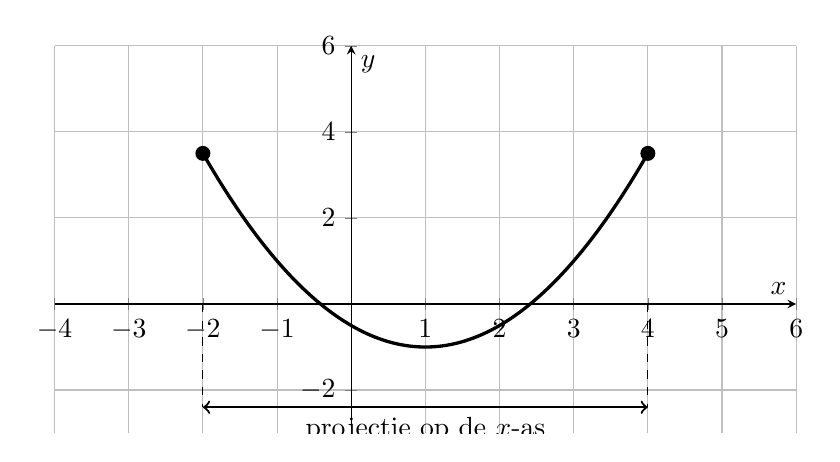
\begin{tikzpicture}
\begin{axis}[
    width=11cm,height=6.5cm,
    xmin=-4,xmax=6,ymin=-3,ymax=6,
    xlabel={$x$},ylabel={$y$},
    axis lines=middle,grid=both,samples=160
]
\addplot[very thick,domain=-2:4] {0.5*(x-1)^2-1};
\addplot[only marks,mark=*,mark size=2.5pt] coordinates {(-2,3.5)(4,3.5)};
\draw[<->,thick] (axis cs:-2,-2.4) -- (axis cs:4,-2.4);
\draw[dashed] (axis cs:-2,0)--(axis cs:-2,-2.4);
\draw[dashed] (axis cs:4,0)--(axis cs:4,-2.4);
\node[below] at (axis cs:1,-2.4) {projectie op de \(x\)-as};
\end{axis}
\end{tikzpicture}
\end{center}

Als we de grafiek evenwijdig met de \(y\)-as op de \(x\)-as projecteren,
zien we voor welke \(x\)-waarden er een punt op de grafiek bestaat.

Hier is
\[
\boxed{\operatorname{dom}f=[-2,4].}
\]
\end{voorbeeld}

\begin{opmerking}
Bij een grafiek moet je aandacht hebben voor eindpunten.

Een \textbf{gevuld punt} behoort tot de grafiek; een \textbf{open punt}
niet. Dat verschil bepaalt of een grenswaarde wel of niet tot het domein behoort.
\end{opmerking}

% ============================================================
% 2. DOMEIN UIT EEN VOORSCHRIFT
% ============================================================

\FVDsubsection{Domein bepalen uit een voorschrift}

Bij een functievoorschrift vertrekken we in principe van alle reële getallen,
maar we verwijderen waarden waarvoor een bewerking niet gedefinieerd is.

Voor de functietypes die we hier nodig hebben, zijn vooral de volgende
voorwaarden belangrijk.

\begin{eigenschap}[Belangrijke domeinvoorwaarden]
\[
\frac{A(x)}{B(x)}
\qquad\Longrightarrow\qquad
B(x)\neq 0,
\]

en

\[
\sqrt{A(x)}
\qquad\Longrightarrow\qquad
A(x)\geq 0.
\]

Wanneer later logaritmische functies worden bestudeerd, komt daar de voorwaarde
bij dat het argument van een logaritme strikt positief moet zijn.
\end{eigenschap}

\begin{voorbeeld}[Een rationale functie]

Gegeven
\[
f(x)=\frac{x+1}{x-3}.
\]

De noemer mag niet nul worden:
\[
x-3\neq0
\quad\Longleftrightarrow\quad
x\neq3.
\]

Dus
\[
\boxed{\operatorname{dom}f=\mathbb{R}\setminus\{3\}.}
\]

\begin{center}
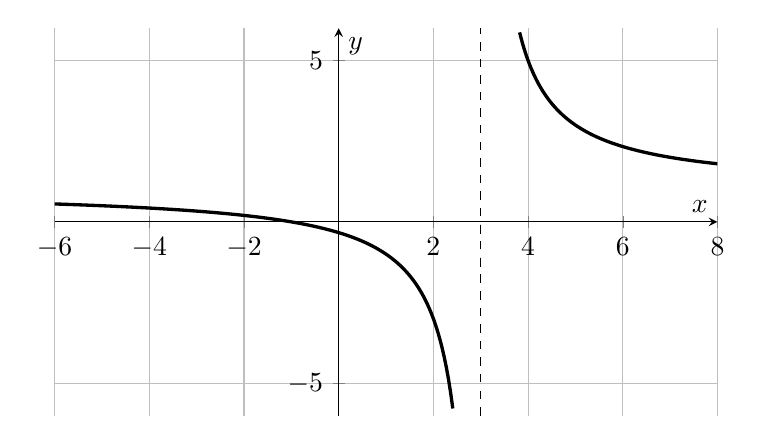
\begin{tikzpicture}
\begin{axis}[
    width=10cm,height=6.5cm,
    xmin=-6,xmax=8,ymin=-6,ymax=6,
    xlabel={$x$},ylabel={$y$},
    axis lines=middle,grid=both,samples=200,
    restrict y to domain=-6:6
]
\addplot[very thick,domain=-6:2.95] {(x+1)/(x-3)};
\addplot[very thick,domain=3.05:8] {(x+1)/(x-3)};
\addplot[dashed,domain=-6:6] ({3},x);
\end{axis}
\end{tikzpicture}
\end{center}

De grafiek bevestigt dat er bij \(x=3\) geen functiewaarde bestaat.
\end{voorbeeld}

\begin{voorbeeld}[Een wortelfunctie]

Gegeven
\[
g(x)=\sqrt{x+2}.
\]

Voor een reële vierkantswortel moet
\[
x+2\geq0.
\]

Dus
\[
\boxed{\operatorname{dom}g=[-2,+\infty[.}
\]

\begin{center}
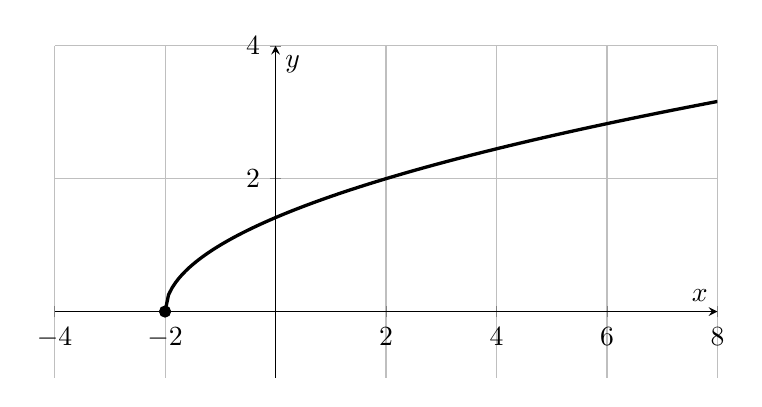
\begin{tikzpicture}
\begin{axis}[
    width=10cm,height=5.8cm,
    xmin=-4,xmax=8,ymin=-1,ymax=4,
    xlabel={$x$},ylabel={$y$},
    axis lines=middle,grid=both,samples=160
]
\addplot[very thick,domain=-2:8] {sqrt(x+2)};
\addplot[only marks,mark=*] coordinates {(-2,0)};
\end{axis}
\end{tikzpicture}
\end{center}
\end{voorbeeld}

% ============================================================
% 3. WISKUNDIG EN PRAKTISCH DOMEIN
% ============================================================

\FVDsubsection{Wiskundig domein en domein in een context}

Een formule kan wiskundig voor meer waarden bestaan dan in een concrete
situatie zinvol zijn.

\begin{definitie}
Het \textbf{praktisch} of \textbf{realistisch domein} is de verzameling
invoerwaarden die binnen de gegeven context mogelijk en zinvol zijn.
\end{definitie}

\begin{voorbeeld}[Hoogte van een bal]

De hoogte van een bal wordt gemodelleerd door
\[
h(t)=1{,}5+8t-4{,}905t^2.
\]

Als zuiver veeltermvoorschrift is deze formule voor iedere reële \(t\) berekenbaar:
\[
\operatorname{dom}h=\mathbb{R}.
\]

Maar wanneer \(t\) de tijd sinds het werpen voorstelt, is \(t<0\) niet zinvol.
Ook nadat de bal de grond raakt, beschrijft dit eenvoudige model de werkelijke
beweging niet verder.

Het realistische domein is dus slechts een deel van \(\mathbb{R}\).

\begin{center}
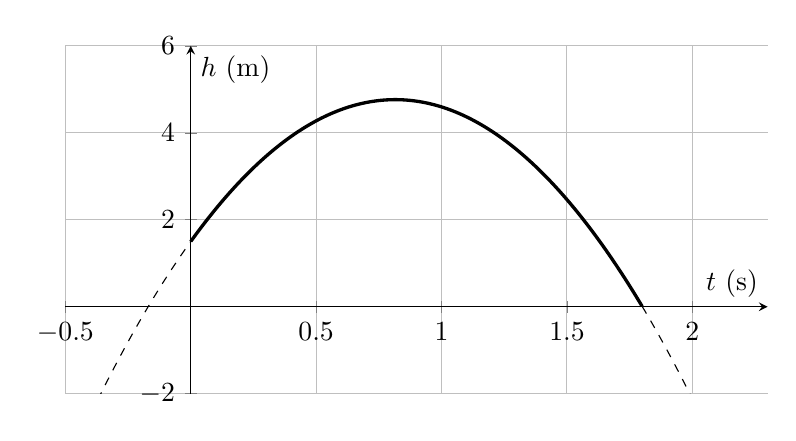
\begin{tikzpicture}
\begin{axis}[
    width=10.5cm,height=6cm,
    xmin=-0.5,xmax=2.3,ymin=-2,ymax=6,
    xlabel={$t$ (s)},ylabel={$h$ (m)},
    axis lines=middle,grid=both,samples=180
]
\addplot[dashed,domain=-0.4:0] {1.5+8*x-4.905*x^2};
\addplot[very thick,domain=0:1.8] {1.5+8*x-4.905*x^2};
\addplot[dashed,domain=1.8:2.2] {1.5+8*x-4.905*x^2};
\end{axis}
\end{tikzpicture}
\end{center}

De wiskunde en de context moeten dus samen gelezen worden.
\end{voorbeeld}

% ============================================================
% 4. BEREIK
% ============================================================

\FVDsection{Het bereik}

\FVDsubsection{Welke uitvoerwaarden worden bereikt? Het bereik}

Het domein kijkt naar de invoer. Het bereik kijkt naar de uitvoer.

\begin{definitie}
Het \textbf{bereik} van een functie \(f\) is de verzameling van alle
functiewaarden die \(f\) werkelijk aanneemt.

We noteren bijvoorbeeld
\[
\operatorname{ber}f.
\]
\end{definitie}
\begin{center} 
    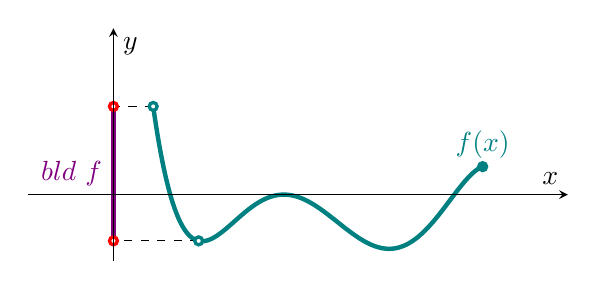
\begin{tikzpicture}

        \begin{axis}[
                    xlabel={$x$},
                    ylabel={$y$},
                    axis equal image=true,
                    grid,
                    grid style={gray!50},
                    grid=both,
                axis y line=center,
                axis x line=middle, 
                axis on top=true,
                xmin=-1.5,
                xmax=8,
                ymin=-2,
                ymax=5,
                xtick={\empty},
                ytick={\empty},
                x=6 cm,
                    ]
            \addplot [domain=0.7:6.5, samples=500, mark=none, ultra thick, teal] {-0.05*(x-1)*(x-3)*(x-3)*(x-6)*(x-7)};
            \draw[violet,ultra thick] (axis cs: 0,-1.39) -- (axis cs: 0,2.65) node[midway,left] {$bld \ f$};
              \draw[dashed] (axis cs: 1.5,-1.39) -- (axis cs: 0,-1.39);
            \draw[dashed] (axis cs: 0.7,2.65) -- (axis cs: 0,2.65);
            \draw[teal, very thick,fill=white]  (axis cs: 0.7,2.65) circle (0.5 mm);
            \draw[red, very thick,fill=white]  (axis cs: 0,2.65) circle (0.5 mm);
            \draw[teal, very thick,fill=white]  (axis cs: 1.5,-1.39) circle (0.5 mm);
            \draw[red, very thick,fill=white]  (axis cs: 0,-1.39) circle (0.5 mm);
            \draw[teal, very thick,fill=teal]  (axis cs: 6.5,0.84) circle (0.5 mm);
          
            \node[teal] at (axis cs:6.5,1.5) {$f(x)$};
            
            
        \end{axis}
        
        
        \end{tikzpicture}
\end{center}

\begin{voorbeeld}[Bereik grafisch bepalen]

Beschouw
\[
f(x)=(x-1)^2-2
\qquad\text{voor}\qquad -2\leq x\leq4.
\]

\begin{center}
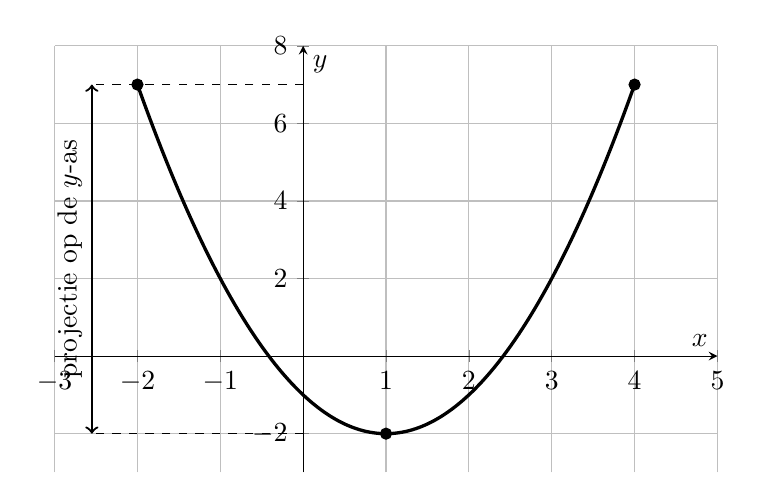
\begin{tikzpicture}
\begin{axis}[
    width=10cm,height=7cm,
    xmin=-3,xmax=5,ymin=-3,ymax=8,
    xlabel={$x$},ylabel={$y$},
    axis lines=middle,grid=both,samples=160
]
\addplot[very thick,domain=-2:4] {(x-1)^2-2};
\addplot[only marks,mark=*] coordinates {(-2,7)(1,-2)(4,7)};
\draw[<->,thick] (axis cs:-2.55,-2)--(axis cs:-2.55,7);
\draw[dashed] (axis cs:0,-2)--(axis cs:-2.55,-2);
\draw[dashed] (axis cs:0,7)--(axis cs:-2.55,7);
\node[rotate=90,above] at (axis cs:-2.55,2.5) {projectie op de \(y\)-as};
\end{axis}
\end{tikzpicture}
\end{center}

De kleinste functiewaarde is \(-2\) en de grootste is \(7\). Alle waarden
daartussen worden bereikt. Dus
\[
\boxed{\operatorname{ber}f=[-2,7].}
\]
\end{voorbeeld}

\begin{opmerking}
Grafisch vinden we het domein door naar de \textbf{horizontale omvang}
van de grafiek te kijken en het bereik door naar de \textbf{verticale omvang}
te kijken.

Denk dus niet alleen aan ``projecteren op een as'', maar vraag:
\begin{itemize}
    \item voor welke \(x\)-waarden bestaat er een punt op de grafiek?
    \item welke \(y\)-waarden komen werkelijk als hoogte van een punt op de grafiek voor?
\end{itemize}
\end{opmerking}

\begin{voorbeeld}[Bereik in een context]

Een tank bevat aanvankelijk \(10\) liter water en wordt gedurende \(12\) minuten
gevuld met \(2\) liter per minuut:
\[
V(t)=10+2t,\qquad 0\leq t\leq12.
\]

Het praktische domein is
\[
[0,12].
\]

Tijdens die periode loopt het volume van \(10\) liter tot \(34\) liter:
\[
\boxed{\operatorname{ber}V=[10,34].}
\]

Het bereik heeft hier dus een concrete betekenis: alle volumes die de tank
tijdens de beschouwde vulperiode aanneemt.
\end{voorbeeld}

% ============================================================
% 5. BEELDEN
% ============================================================

\FVDsubsection{Van invoer naar uitvoer: beelden}

\begin{definitie}
Als \(a\) tot het domein van \(f\) behoort, dan noemen we
\[
f(a)
\]
het \textbf{beeld} van \(a\) door \(f\).
\end{definitie}

\begin{voorbeeld}
Voor
\[
f(x)=x^2-2x
\]
is
\[
f(3)=3^2-2\cdot3=3.
\]

Dus \(3\) is het beeld van \(3\) door \(f\).
\end{voorbeeld}

Grafisch vertrekken we van de invoerwaarde op de \(x\)-as, bewegen verticaal
naar de grafiek en daarna horizontaal naar de \(y\)-as.

\begin{center}
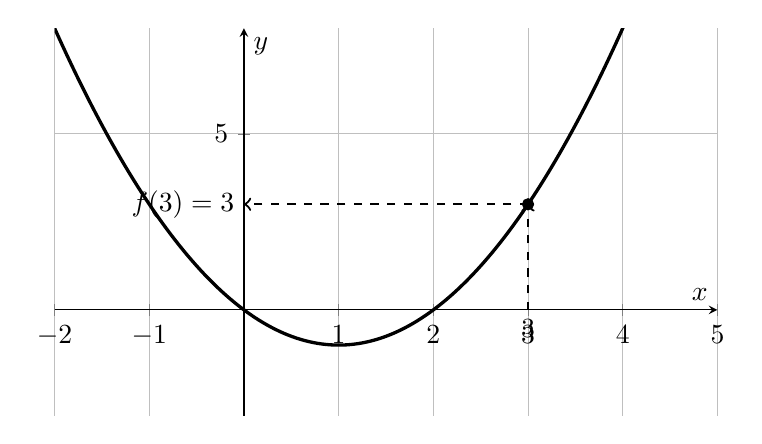
\begin{tikzpicture}
\begin{axis}[
    width=10cm,height=6.5cm,
    xmin=-2,xmax=5,ymin=-3,ymax=8,
    xlabel={$x$},ylabel={$y$},
    axis lines=middle,grid=both,samples=160
]
\addplot[very thick,domain=-2:5] {x^2-2*x};
\addplot[only marks,mark=*] coordinates {(3,3)};
\draw[->,thick,dashed] (axis cs:3,0)--(axis cs:3,3);
\draw[->,thick,dashed] (axis cs:3,3)--(axis cs:0,3);
\node[below] at (axis cs:3,0) {$3$};
\node[left] at (axis cs:0,3) {$f(3)=3$};
\end{axis}
\end{tikzpicture}
\end{center}

% ============================================================
% 6. ORIGINELEN
% ============================================================

\FVDsection{Van uitvoer terug naar invoer: originelen}

We kunnen de vraag ook omkeren.

In plaats van
\[
\text{``Wat is het beeld van \(a\)?''}
\]
vragen we
\[
\text{``Welke invoerwaarden hebben beeld \(b\)?''}
\]

\begin{definitie}
Een getal \(a\) is een \textbf{origineel} van \(b\) door de functie \(f\)
als
\[
f(a)=b.
\]
\end{definitie}

Een functiewaarde kan geen, één of meerdere originelen hebben.

\begin{voorbeeld}[Meerdere originelen]

Gegeven
\[
f(x)=x^2.
\]

Zoek de originelen van \(4\).

We lossen op:
\[
f(x)=4
\]
dus
\[
x^2=4.
\]

Daaruit volgt
\[
x=-2\qquad\text{of}\qquad x=2.
\]

Het getal \(4\) heeft dus twee originelen.

\begin{center}
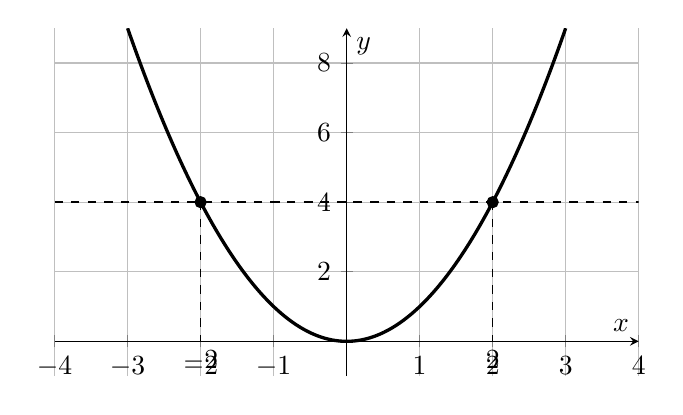
\begin{tikzpicture}
\begin{axis}[
    width=9cm,height=6cm,
    xmin=-4,xmax=4,ymin=-1,ymax=9,
    xlabel={$x$},ylabel={$y$},
    axis lines=middle,grid=both,samples=160
]
\addplot[very thick,domain=-3:3] {x^2};
\addplot[thick,dashed,domain=-4:4] {4};
\addplot[only marks,mark=*] coordinates {(-2,4)(2,4)};
\draw[dashed] (axis cs:-2,4)--(axis cs:-2,0);
\draw[dashed] (axis cs:2,4)--(axis cs:2,0);
\node[below] at (axis cs:-2,0) {$-2$};
\node[below] at (axis cs:2,0) {$2$};
\end{axis}
\end{tikzpicture}
\end{center}

Grafisch zoeken we originelen van \(b\) door de horizontale lijn
\[
y=b
\]
te tekenen en de \(x\)-coördinaten van de snijpunten te bepalen.
\end{voorbeeld}

\begin{opmerking}[Vooruit en terug]
Bij een functie is de richting
\[
x\longrightarrow f(x)
\]
altijd eenduidig.

De omgekeerde vraag
\[
y\longrightarrow \text{origineel(en)}
\]
hoeft niet eenduidig te zijn.

Dit onderscheid wordt in het volgende hoofdstuk belangrijk wanneer we onderzoeken
wanneer een functie \textbf{omkeerbaar} is.
\end{opmerking}

% ============================================================
% 7. DOMEIN, CODOMEIN EN BEREIK
% ============================================================

\FVDsection{Domein, codomein en bereik}

Om later bijectie en inverse functies correct te kunnen beschrijven,
hebben we nog één begrip nodig.

\begin{definitie}
Bij een functie
\[
f:A\to B
\]
noemen we:
\begin{itemize}
    \item \(A\) het \textbf{domein};
    \item \(B\) het \textbf{codomein};
    \item de werkelijk aangenomen functiewaarden het \textbf{bereik}.
\end{itemize}
\end{definitie}

Het bereik ligt dus in het codomein:
\[
\operatorname{ber}f\subseteq B.
\]

\begin{voorbeeld}
Beschouw
\[
f:\mathbb{R}\to\mathbb{R}:x\mapsto x^2.
\]

Dan is
\[
\operatorname{dom}f=\mathbb{R},
\qquad
\text{codomein}=\mathbb{R},
\qquad
\operatorname{ber}f=[0,+\infty[.
\]

Negatieve reële getallen behoren wel tot het codomein, maar worden door deze
functie nooit als functiewaarde bereikt.
\end{voorbeeld}

\begin{opmerking}
Het onderscheid tussen codomein en bereik wordt hier alleen ingevoerd omdat
het noodzakelijk is om in het volgende hoofdstuk \textbf{surjectiviteit} en
\textbf{bijectie} correct te begrijpen. We bouwen er geen afzonderlijke
verzamelingenleer rond.
\end{opmerking}

% ============================================================
% 8. GEOGEBRA
% ============================================================

\FVDsection{Onderzoeken met GeoGebra}

GeoGebra kan domein en bereik zichtbaar maken, maar het programma vervangt
de redenering niet.

\begin{fvdgeogebra}[Domein, bereik en originelen onderzoeken]

    Voer in GeoGebra de functies
    
    \[
    f(x)=\sqrt{x+2},
    \qquad
    g(x)=\frac{x+1}{x-3},
    \qquad
    h(x)=(x-1)^2-2.
    \]
    
    Onderzoek voor elke functie:
    
    \begin{enumerate}
    
        \item Voor welke \(x\)-waarden zie je punten op de grafiek?
    
        \item Welke \(y\)-waarden worden bereikt?
    
        \item Kan je het domein verklaren vanuit het functievoorschrift?
    
        \item Kies een waarde \(b\) en teken de horizontale lijn
        \[
        y=b.
        \]
        Hoeveel originelen heeft \(b\)?
    
        \item Verander \(b\). Wanneer verandert het aantal originelen?
    
    \end{enumerate}
    
    Gebruik de grafiek eerst om een vermoeden te formuleren.
    Verklaar daarna waar mogelijk algebraïsch waarom je waarneming klopt.
    
    \end{fvdgeogebra}

% ============================================================
% 9. STEM-CONTEXT
% ============================================================

\FVDsection{Toepassingen}

\begin{voorbeeld}[Elektrisch vermogen in een weerstand]

Voor een weerstand \(R>0\) geldt
\[
P=RI^2,
\]
waarbij \(P\) het elektrisch vermogen en \(I\) de stroomsterkte is.

Neem \(R=15\,\Omega\). Dan
\[
P(I)=15I^2.
\]

Als we in een proef alleen stroomsterkten tussen \(0\) A en \(2\) A toelaten,
is het praktische domein
\[
[0,2].
\]

Het vermogen loopt dan van
\[
P(0)=0
\]
tot
\[
P(2)=60.
\]

Dus
\[
\operatorname{ber}P=[0,60]
\]
binnen deze proefopstelling.

\begin{center}
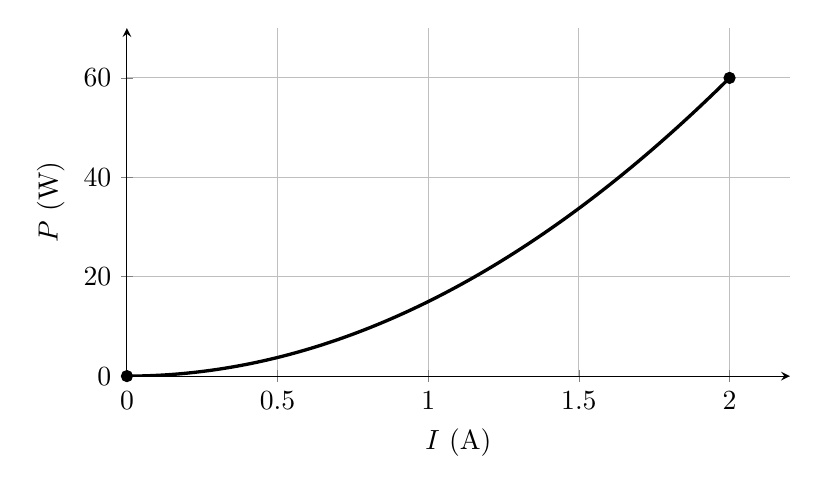
\begin{tikzpicture}
\begin{axis}[
    width=10cm,height=6cm,
    xmin=0,xmax=2.2,ymin=0,ymax=70,
    xlabel={$I$ (A)},ylabel={$P$ (W)},
    axis lines=left,grid=both,samples=160
]
\addplot[very thick,domain=0:2] {15*x^2};
\addplot[only marks,mark=*] coordinates {(0,0)(2,60)};
\end{axis}
\end{tikzpicture}
\end{center}

Merk op dat domein en bereik hier niet alleen wiskundige verzamelingen zijn:
ze beschrijven welke waarden in de proef worden toegelaten en welke
vermogens daarbij kunnen optreden.
\end{voorbeeld}



\end{document}
